%%% Copyright (C) 2017 Vincent Goulet
%%%
%%% This file and all files included or input by this one (and
%%% recursively) are part of the project "The Best of Both Worlds:
%%% Using Blended Learning in Actuarial Science Courses - Actuarial
%%% Teaching Conference 2017"
%%% http://github.com/vigou3/ATC2017-blended-learning
%%%
%%% This work is licensed under a Creative Commons
%%% Attribution-ShareAlike 4.0 International License.
%%% http://creativecommons.org/licenses/by-sa/4.0/

\documentclass[aspectratio=1610,10pt,xcolor=x11names]{beamer}
  \usepackage[round]{natbib}
  \usepackage{fontawesome}
  \usepackage{changepage}                % page licence
  \usepackage{tabularx}                  % page licence
  \usepackage{framed}                    % env. leftbar
  \usepackage[export]{adjustbox}         % cadre autour image
  \usepackage[overlay,absolute]{textpos} % covers
  \usepackage{metalogo}                  % logo \XeLaTeX

  %% ==================
  %%  Publication info
  %% ==================
  \renewcommand{\year}{2017}

  %% ===============================
  %%  Look and feel of the document
  %% ===============================

  %% Beamer theme
  \usetheme{metropolis}

  %% Additionnal colors
  \definecolor{link}{rgb}{0,0.4,0.6}        % internal links
  \definecolor{url}{rgb}{0.6,0,0}           % external links
  \definecolor{rouge}{rgb}{0.85,0,0.07}     % UL red stripe
  \definecolor{or}{rgb}{1,0.8,0}            % UL yellow stripe
  \colorlet{alert}{mLightBrown} % alias for Metropolis color
  \colorlet{dark}{mDarkTeal}    % alias for Metropolis color

  %% Hyperlinks
  \hypersetup{%
    pdfauthor = {Vincent Goulet},
    pdftitle = {The Best of Both Worlds: Using Blended Learning in Actuarial Science Courses},
    colorlinks = {true},
    linktocpage = {true},
    allcolors = {link},
    urlcolor = {url},
    pdfpagemode = {UseOutlines},
    pdfstartview = {Fit},
    bookmarksopen = {true},
    bookmarksnumbered = {true},
    bookmarksdepth = {subsection}}

  %% Bibliography
  %% Couple of hacks needed to have beamer and natbib play nice with
  %% each other.
  \renewcommand{\newblock}{}    % https://tex.stackexchange.com/a/1971/24355
  \renewcommand{\bibsection}{}  % drop \section heading
  \bibliographystyle{abbrvnat}

  %% =====================
  %%  Nouvelles commandes
  %% =====================

  \newcommand{\link}[2]{\href{#1}{#2~\raisebox{-0.2ex}{\faExternalLink}}}
  \newcommand{\meta}[1]{\ensuremath\langle{\normalfont\itshape #1\/}\ensuremath\rangle}

  %% Link to GitHub on copyright page
  \newcommand{\viewsource}[1]{%
    \href{#1}{%
      \makebox[2.5mm]{\raisebox{-1pt}{\footnotesize\faGithub}}\;%
      {\sffamily View on GitHub}}}

  %%% =======
  %%%  Varia
  %%% =======

  %% Lengths used to compose front and rear covers.
  \newlength{\banderougewidth} \newlength{\banderougeheight}
  \newlength{\bandeorwidth}    \newlength{\bandeorheight}
  \newlength{\imageheight}     \newlength{\imagewidth}
  \newlength{\logoheight}
  \newlength{\gapwidth}

%  \includeonly{couverture-avant}

\begin{document}

%% frontmatter
\begingroup

\TPGrid{3}{36}
\textblockorigin{0mm}{0mm}
\setlength{\parindent}{0mm}
\setlength{\banderougewidth}{2\TPHorizModule}
\setlength{\banderougeheight}{\TPVertModule}
\setlength{\bandeorwidth}{\TPHorizModule}
\setlength{\bandeorheight}{\banderougeheight}
\setlength{\imageheight}{29\TPVertModule}
\setlength{\imagewidth}{3\TPHorizModule}
\setlength{\logoheight}{2.5\TPVertModule}
\setlength{\gapwidth}{0.75pt}
\addtolength{\bandeorwidth}{-\gapwidth}
\addtolength{\imageheight}{-\gapwidth}

\begin{frame}[plain]
  %% UL banner
  \begin{textblock*}{3\TPHorizModule}[0,1](0mm,30\TPVertModule)
    \textcolor{rouge}{\rule{\banderougewidth}{\banderougeheight}}% % red stripe
    \rule{\gapwidth}{0pt}%                                         % gap
    \textcolor{or}{\rule{\bandeorwidth}{\bandeorheight}}           % gold stripe
  \end{textblock*}

  %% UL logo
  \begin{textblock*}{\TPHorizModule}(2\TPHorizModule,31\TPVertModule)
    \rule{\gapwidth}{0pt}%                                     % gap
    \includegraphics[height=\logoheight,keepaspectratio=true]{ul_p}
  \end{textblock*}

  %% background image
  \begin{textblock*}{3\TPHorizModule}(0mm,0mm)
    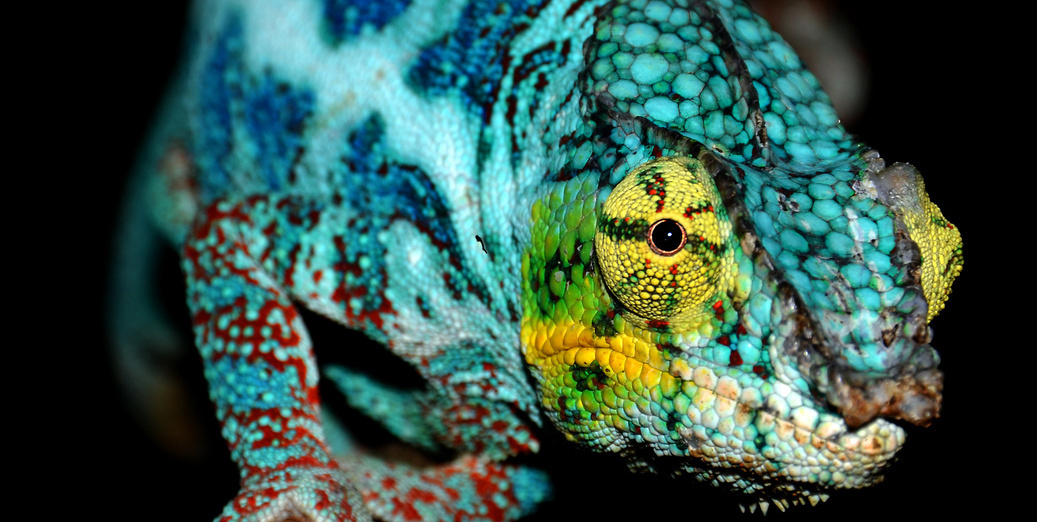
\includegraphics[height=\imageheight,width=\imagewidth]{furcifer-pardalis-nosy-faly}
  \end{textblock*}

  %% title
  \begin{textblock*}{2\TPHorizModule}(0.205\TPHorizModule,3.1\TPVertModule)
    %% Poor Man's (but simple!) shadow effect behind letters; needed
    %% to let the title stand out on the dark background
    \raggedright%
    \bfseries
    \fontsize{20}{20}\selectfont
    \textcolor{black}{%
      The Best of Both Worlds: \\
      Using Blended Learning \\
      in Actuarial Science Courses} \\
    \mdseries
    \fontsize{14}{18}\selectfont
    \textcolor{black}{Actuarial Teaching Conference 2017}
  \end{textblock*}
  \begin{textblock*}{2\TPHorizModule}(0.2\TPHorizModule,3\TPVertModule)
    \raggedright%
    \bfseries
    \fontsize{20}{20}\selectfont
    \textcolor{white}{%
      The Best of Both Worlds: \\
      Using Blended Learning \\
      in Actuarial Science Courses} \\
    \mdseries
    \fontsize{14}{18}\selectfont
    \textcolor{white}{Actuarial Teaching Conference 2017}
  \end{textblock*}

  %% date
  \begin{textblock*}{2\TPHorizModule}(0.2\TPHorizModule,26\TPVertModule)
    \fontsize{10}{12}\selectfont
    \textcolor{white}{June 27, 2017}
  \end{textblock*}
\end{frame}
\endgroup

%%% Local Variables:
%%% mode: latex
%%% TeX-engine: xetex
%%% TeX-master: "ATC2017-blended-learning"
%%% End:

\begingroup

\TPGrid{3}{36}
\textblockorigin{0mm}{0mm}
\begin{frame}[plain]
  %% title
  \begin{textblock*}{2\TPHorizModule}(0.2\TPHorizModule,3\TPVertModule)
    \raggedright%
    \bfseries
    \fontsize{20}{20}\selectfont
    The Best of Both Worlds: \\
    Using Blended Learning \\
    in Actuarial Science Courses \\
    \mdseries
    \fontsize{14}{18}\selectfont
    Actuarial Teaching Conference 2017
  \end{textblock*}

  %% author
  \begin{textblock*}{2\TPHorizModule}(0.2\TPHorizModule,17\TPVertModule)
    \fontsize{10}{11}\selectfont
    \bfseries
    Vincent Goulet \\
    \fontsize{9}{11}\selectfont
    \mdseries
    École d'actuariat, Université Laval
  \end{textblock*}
\end{frame}
\endgroup

%%% Local Variables:
%%% mode: latex
%%% TeX-engine: xetex
%%% TeX-master: "atc-2017-blended-learning"
%%% End:

%%% Texte du contrat de licence au début des diapos

\begin{frame}[t,plain,fragile=singleslide]
  \tiny
  \vspace*{10mm}

  \begin{adjustwidth}{15mm}{15mm}
    {\textcopyright} {\year} Vincent Goulet \\[4mm]

    
\includegraphics[height=4mm,keepaspectratio=true]{by-sa} \\%

    This work is licensed under a Creative Commons
    \href{http://creativecommons.org/licenses/by-sa/4.0/deed.en}{%
      Attribution-ShareAlike 4.0 International}
    license. You are free to:
    \begin{itemize}
    \item \textbf{Share} --- copy and redistribute the material in any
      medium or format;
    \item \textbf{Adapt} --- remix, transform, and build upon the
      material for any purpose, even commercially.
    \end{itemize}
    Under the following terms: \vspace*{2mm}

    \begin{tabularx}{\linewidth}{@{}lX@{}}
      \raisebox{-5.5mm}[0mm][7mm]{%
        
\includegraphics[height=7mm,keepaspectratio=true]{by}} &
      \textbf{Attribution} --- You must give appropriate credit,
      provide a link to the license, and indicate if changes were
      made. You may do so in any reasonable manner, but not in any way
      that suggests the licensor endorses you or your use. \\
      \raisebox{-5.5mm}{
\includegraphics[height=7mm,keepaspectratio=true]{sa}}
      & \textbf{ShareAlike} --- If you remix, transform, or build upon
      the material, you must distribute your contributions under the
      same license as the original. \\
      & \textbf{No additional restrictions} --— You may not apply
      legal terms or technological measures that legally restrict
      others from doing anything the license permits.
    \end{tabularx}
    \vspace{5mm}

    \textbf{Source code} \\
    \viewsource{https://github.com/vigou3/ATC2017-blended-learning/}

    \textbf{Photo credit} \\
    Stefan Overmann; \url{http://fc-foto.de/32711819}
  \end{adjustwidth}
\end{frame}

%%% Local Variables:
%%% mode: latex
%%% TeX-engine: xetex
%%% TeX-master: "ATC2017-blended-learning"
%%% End:


%% mainmatter

\section{Teaching in a Digital Age}

\begin{frame}
  \centering
  From heavy note taking sessions\dots \\
  \begin{minipage}{0.55\linewidth}
    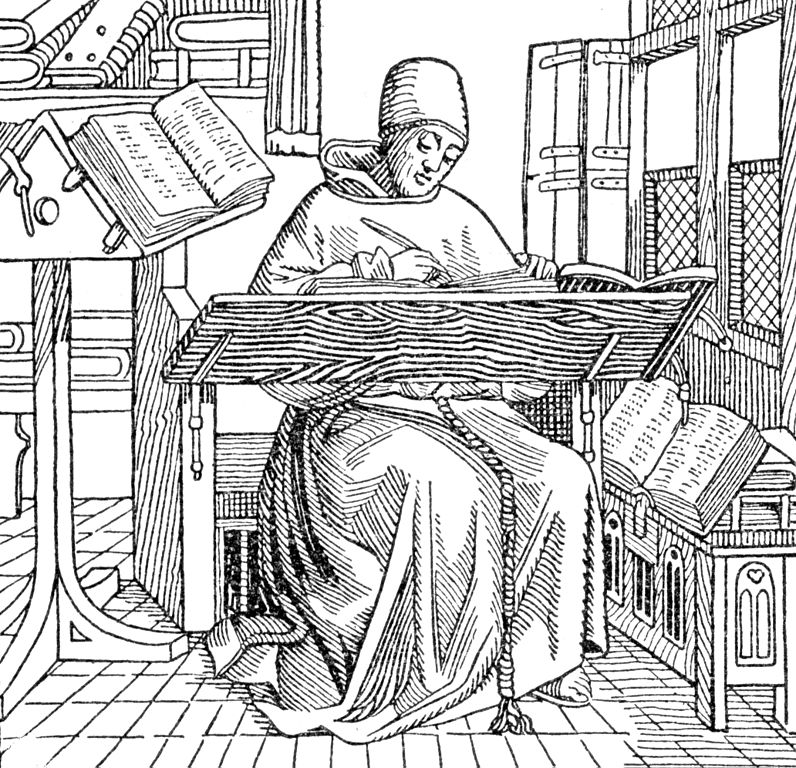
\includegraphics[width=\linewidth,keepaspectratio]{796px-Monkcopyistwoodcut} \\
    \tiny \href{https://commons.wikimedia.org/wiki/File:Monkcopyistwoodcut.jpg}{Wikimedia Commons}
  \end{minipage}
\end{frame}

\begin{frame}
  \centering
  \dots\ to PowerPoint Syndrome \\
  \begin{minipage}{\linewidth}
    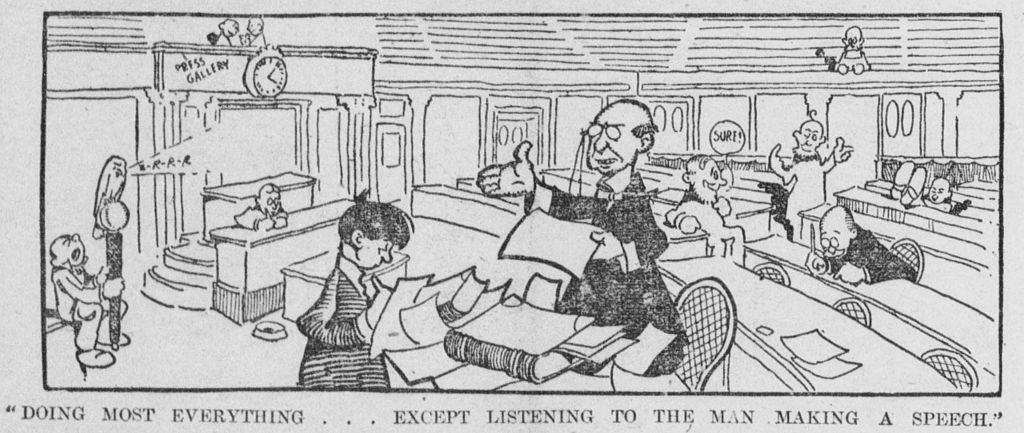
\includegraphics[width=\linewidth,keepaspectratio]{Satterfield_watches_Congress_be_boring} \\
    \tiny \href{https://commons.wikimedia.org/wiki/File:Satterfield_watches_Congress_be_boring.jpg}{Wikimedia Commons}
  \end{minipage}
\end{frame}

\begin{frame}
  \begin{center}
    \textbf{Late 2000s}
  \end{center}
  \begin{center}
    The classroom is obsolete! \\
    \emph{e-learning} is the future!
  \end{center}
\end{frame}

\begin{frame}
  \begin{center}
    \textbf{Pendulum is swinging back}
  \end{center}
  \begin{center}
    Students like to meet their teacher \\
    \pause
    \dots\ provided it's worth it.
  \end{center}
\end{frame}

\begin{frame}[standout]
  Disclaimer \\
  \bigskip

  I am not a specialist.

  Just an ordinary professor\dots \\
  with some experience
\end{frame}

\section{Blended Learning: \newline Identification and Taxonomy}

\begin{frame}
  \frametitle{Definition (One of Many)}

  \begin{quote}
    Thoughtful fusion of face-to-face and online learning experiences
    [\dots] optimally integrated such that \alert{the strengths of
      each} are blended into a unique learning experience congruent
    with the context and intended educational purpose.
    \citep{Garrison:blended:2007}
  \end{quote}
\end{frame}

\begin{frame}
  \frametitle{Models of Blended Learning}

  \begin{description}[Enriched-virtual model]
  \item[Rotation model] Online engagement embedded within face-to-face
    forms of instruction in a cyclical manner
  \item[Flex model] Multiple students engaged primarily online, but
    under the supervision of a teacher who is physically present
  \item[Self-blending model] Students choose different courses to take
    independently, but do so in a setting where a supervising teacher
    and other students are co-present
  \item[\alert<2>{Enriched-virtual model}] Online, virtual experiences are seen
    as being enriched only periodically through arrangements of
    physical co-presence
  \end{description}

  {\tiny \citep{Stalker:blended:2012,Friesen:blended:2012}}
\end{frame}

\begin{frame}
  \frametitle{Continuum of Technology-Based Learning}

  \centering
  \begin{minipage}{0.75\linewidth}
    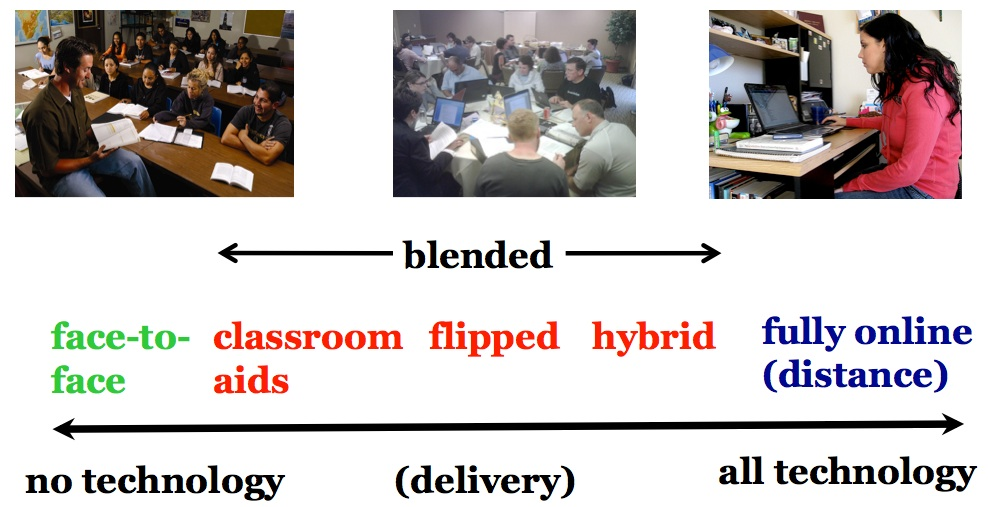
\includegraphics[width=\linewidth,keepaspectratio]{Continuum-of-technology-based-teaching-2} \\
    \tiny \citep{Bates:digital:2015}
  \end{minipage}
  \vfill
  \mbox{}

  \setlength{\unitlength}{1mm}
  \only<2->{
    \begin{textblock*}{0mm}(80mm,78mm)
      \begin{picture}(0,0)
        \put(-8,21){\framebox(16,6.5)[bl]{}}
        \put(0,-7){\line(0,1){28}}
        \put(-41,-2){%
          \parbox[t]{40mm}{%
            \small\raggedleft%
            lectures prepared online before meeting in class}}
      \end{picture}
    \end{textblock*}}

  \only<3->{
    \begin{textblock*}{0mm}(97mm,78mm)
      \begin{picture}(0,0)
        \put(-8,21){\framebox(16,6.5)[bl]{}}
        \put(0,-16){\line(0,1){37}}
        \put(1,-2){%
          \parbox[t]{50mm}{%
            \small\raggedright%
            majority of learning online, class only for very specific
            face-to-face teaching that cannot be done satisfactorily online}}
      \end{picture}
    \end{textblock*}}
\end{frame}


\section{How I Stopped Worrying \newline and Love Blended Learning}

\begin{frame}[fragile=singleslide]
  \frametitle{Context}

  \begin{itemize}
  \item Numerical Methods course with R Programming component
  \item Teaching of programming part further \alert{left} on the blended
    learning continuum
    \begin{center}
      \medskip
      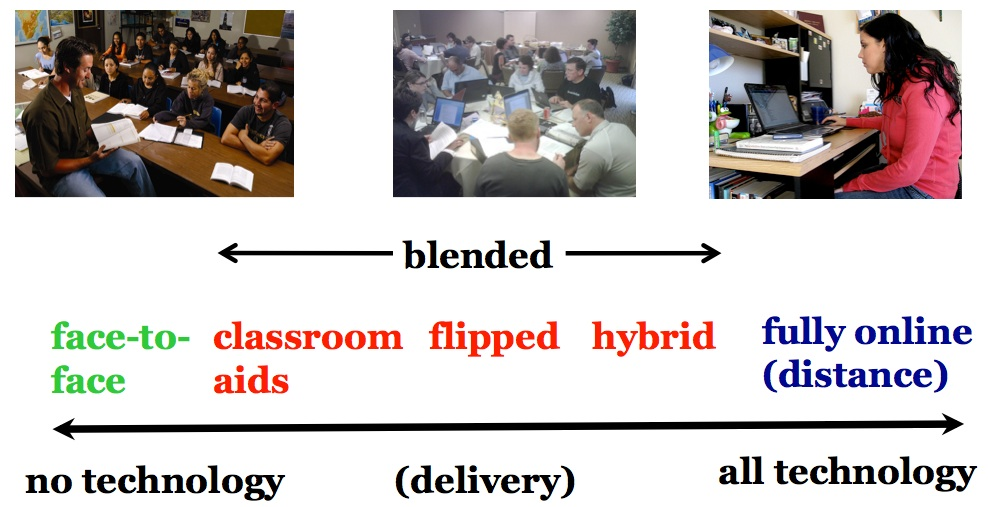
\includegraphics[width=0.7\linewidth,keepaspectratio,%
        trim=0 0 0 230,clip]{Continuum-of-technology-based-teaching-2}
      \setlength{\unitlength}{1mm}
      \begin{picture}(0,0)
        \put(-75,10){\framebox(19.8,8)[bl]{}}
      \end{picture}
    \end{center}

  \item Strong push towards fully online (distance) learning at Université Laval
  \end{itemize}
\end{frame}

\begin{frame}
  \frametitle{Motivation}

  \begin{itemize}
  \item \alert{Not} to increase course accessibility
  \item Administrative duties
    \begin{itemize}
    \item looking for a more free-standing course
    \end{itemize}
  \item Ineffectiveness of assignments
    \begin{itemize}
    \item no feedback to students
    \item complaints about workload
    \end{itemize}
  \end{itemize}
\end{frame}

%% These are defined outside the following frame to avoid troubles
%% with overlays.
\setlength{\unitlength}{1mm}
\newsavebox{\activity}
\savebox{\activity}(4,0){\color{alert}\circle*{4}}
\newsavebox{\week}
\savebox{\week}(12,0){\color{dark}\rule[-1mm]{12mm}{2mm}}

\begin{frame}
  \frametitle{My Hybrid Teaching Model}
  \centering
  \begin{picture}(125,60)
    \put(0,40){\usebox{\activity}}
    \put(4,40){\usebox{\week}}
    \put(18,40){\usebox{\week}} \put(30,40){\usebox{\activity}}
    \put(34,40){\usebox{\week}} \put(46,40){\usebox{\activity}}
    \put(50,40){\usebox{\week}}
    \put(64,40){\usebox{\week}} \put(70,44){\makebox(0,0){\color{alert}\faPlusSquare}}
    \put(78,40){\usebox{\week}} \put(90,40){\usebox{\activity}}
    \put(94,40){\usebox{\week}}
    \multiput(109,40)(2.5,0){3}{\circle*{0.7}}

    \only<2->{
      \put(0,37.5){\line(0,-1){31}}
      \put(1,30){%
        \begin{minipage}[t]{35mm}
          \faUsers \\ Launch activity
          \begin{itemize}
          \item welcome
          \item course outline
          \item software install
          \end{itemize}
        \end{minipage}}
    }

    \only<3->{
      \put(40,37.5){\line(0,-1){31}}
      \put(41,30){%
        \begin{minipage}[t]{50mm}
          \faUser \\ Independent work
          \begin{itemize}
          \item theory and examples
          \item exercices
          \item formative assessments
          \end{itemize}
        \end{minipage}}
    }

    \only<4->{
      \put(90,37.5){\line(0,-1){26}}
      \put(91,30){%
        \begin{minipage}[t]{35mm}
          \faUsers \\ Classroom activities
          \begin{itemize}
          \item review of material
          \item team project
          \end{itemize}
        \end{minipage}}
    }

    \only<5->{
      \put(70,46.2){\line(0,1){12}}
      \put(71,50){%
        \parbox[b]{30mm}{\faShareAlt \\ Online tutorial}}
    }
  \end{picture}
\end{frame}

\section{Demo}

\section{Field Report}

\begin{frame}
  \frametitle{Students Feedback}

  \begin{minipage}{0.48\textwidth}
    They like
    \begin{itemize}
    \item Autonomy
    \item Flexible schedule
    \item Variety of learning experiences
    \end{itemize}
  \end{minipage}
  \hfill
  \begin{minipage}{0.48\textwidth}
    They like less
    \begin{itemize}
    \item Autonomy
    \item Apparent lack of supervision
    \item Time constrained (60~min.) projects
    \end{itemize}
  \end{minipage}
\end{frame}

\begin{frame}
  \frametitle{Tips and Tricks}

  \begin{itemize}[<+->]
  \item Trust the students
  \item Don't trust the students ;-)
  \end{itemize}

  \begin{itemize}[<3->]
  \item Plan, starting from learning objectives
  \item Provide a clear roadmap
  \item Vary learning experiences
  \item Write exam questions congruent with learning objectives
  \item Avoid overengineering
  \end{itemize}

  \begin{itemize}[<4->]
  \item You will need a learning management system (LMS)
  \end{itemize}
\end{frame}

%%% Local Variables:
%%% mode: latex
%%% TeX-engine: xetex
%%% TeX-master: "atc-2017-blended-learning"
%%% End:


%% backmatter
\begin{frame}
  \frametitle{References}
  \small

  \nocite{Bates:10fundamentals:2016,Friesen:lecture:2016}

  \bibliography{education}
\end{frame}

%%% Local Variables:
%%% mode: latex
%%% TeX-engine: xetex
%%% TeX-master: "atc-2017-blended-learning"
%%% End:

\begin{frame}[plain]
  \begin{adjustwidth}{20mm}{20mm}
    \scriptsize \raggedright %
    This document was typeset with {\XeLaTeX} using the
    \textbf{beamer} class and the Metropolis theme. The text is in
    Fira Sans and icons come from Font~Awesome.
  \end{adjustwidth}
\end{frame}

%%% Local Variables:
%%% mode: latex
%%% TeX-engine: xetex
%%% TeX-master: "atc-2017-blended-learning"
%%% End:

\begingroup

\TPGrid{3}{36}
\textblockorigin{0mm}{0mm}
\setlength{\parindent}{0mm}
\setlength{\banderougewidth}{2\TPHorizModule}
\setlength{\bandeorwidth}{\TPHorizModule}
\setlength{\gapwidth}{0.75pt}
\addtolength{\bandeorwidth}{-\gapwidth}

\begin{frame}[plain]
  \begin{textblock*}{125mm}[0,1](0mm,30\TPVertModule)
    \textcolor{or}{\rule{\bandeorwidth}{\TPVertModule}}%      % gold stripe
    \rule{\gapwidth}{0pt}%                                    % gap
    \textcolor{rouge}{\rule{\banderougewidth}{\TPVertModule}} % red stripe
  \end{textblock*}
\end{frame}
\endgroup

%%% Local Variables:
%%% mode: latex
%%% TeX-engine: xetex
%%% TeX-master: "atc-2017-blended-learning"
%%% End:


\end{document}

%%% Local Variables:
%%% mode: latex
%%% TeX-engine: xetex
%%% TeX-master: t
%%% End:
